%%
%% This is file `sample-sigconf-authordraft.tex',
%% generated with the docstrip utility.
%%
%% The original source files were:
%%
%% samples.dtx  (with options: `all,proceedings,bibtex,authordraft')
%% 
%% IMPORTANT NOTICE:
%% 
%% For the copyright see the source file.
%% 
%% Any modified versions of this file must be renamed
%% with new filenames distinct from sample-sigconf-authordraft.tex.
%% 
%% For distribution of the original source see the terms
%% for copying and modification in the file samples.dtx.
%% 
%% This generated file may be distributed as long as the
%% original source files, as listed above, are part of the
%% same distribution. (The sources need not necessarily be
%% in the same archive or directory.)
%%
%%
%% Commands for TeXCount
%TC:macro \cite [option:text,text]
%TC:macro \citep [option:text,text]
%TC:macro \citet [option:text,text]
%TC:envir table 0 1
%TC:envir table* 0 1
%TC:envir tabular [ignore] word
%TC:envir displaymath 0 word
%TC:envir math 0 word
%TC:envir comment 0 0
%%
%% The first command in your LaTeX source must be the \documentclass
%% command.
%%
%% For submission and review of your manuscript please change the
%% command to \documentclass[manuscript, screen, review]{acmart}.
%%
%% When submitting camera ready or to TAPS, please change the command
%% to \documentclass[sigconf]{acmart} or whichever template is required
%% for your publication.
%%
%%
\documentclass[sigconf,authordraft]{acmart}
\usepackage{listings}
%%
%% \BibTeX command to typeset BibTeX logo in the docs
\AtBeginDocument{%
  \providecommand\BibTeX{{%
    Bib\TeX}}}

%% Rights management information.  This information is sent to you
%% when you complete the rights form.  These commands have SAMPLE
%% values in them; it is your responsibility as an author to replace
%% the commands and values with those provided to you when you
%% complete the rights form.
\setcopyright{acmlicensed}
\copyrightyear{2024}
\acmYear{2024}
%% These commands are for a PROCEEDINGS abstract or paper.
\acmConference[Computação Natural]{Computação Natural}{February 05,
  2025}{Belo Horizonte, MG, Brazil}
%%
%%  Uncomment \acmBooktitle if the title of the proceedings is different
%%  from ``Proceedings of ...''!
%%
%%\acmBooktitle{Woodstock '18: ACM Symposium on Neural Gaze Detection,
%%  June 03--05, 2018, Woodstock, NY}
% \acmISBN{978-1-4503-XXXX-X/2018/06}


%%
%% Submission ID.
%% Use this when submitting an article to a sponsored event. You'll
%% receive a unique submission ID from the organizers
%% of the event, and this ID should be used as the parameter to this command.
%%\acmSubmissionID{123-A56-BU3}

%%
%% For managing citations, it is recommended to use bibliography
%% files in BibTeX format.
%%
%% You can then either use BibTeX with the ACM-Reference-Format style,
%% or BibLaTeX with the acmnumeric or acmauthoryear sytles, that include
%% support for advanced citation of software artefact from the
%% biblatex-software package, also separately available on CTAN.
%%
%% Look at the sample-*-biblatex.tex files for templates showcasing
%% the biblatex styles.
%%

%%
%% The majority of ACM publications use numbered citations and
%% references.  The command \citestyle{authoryear} switches to the
%% "author year" style.
%%
%% If you are preparing content for an event
%% sponsored by ACM SIGGRAPH, you must use the "author year" style of
%% citations and references.
%% Uncommenting
%% the next command will enable that style.
%%\citestyle{acmauthoryear}


%%
%% end of the preamble, start of the body of the document source.
\begin{document}

%%
%% The "title" command has an optional parameter,
%% allowing the author to define a "short title" to be used in page headers.
\title{Using Genetic Algorithms to Optimize Hashcat Masks}

%%
%% The "author" command and its associated commands are used to define
%% the authors and their affiliations.
%% Of note is the shared affiliation of the first two authors, and the
%% "authornote" and "authornotemark" commands
%% used to denote shared contribution to the research.
\author{Rafael Dias Campos}
\affiliation{
  \institution{Universidade Federal de Minas Gerais}
  \city{Belo Horizonte}
  \state{Minas Gerais}
  \country{Brasil}
}

%%
%% By default, the full list of authors will be used in the page
%% headers. Often, this list is too long, and will overlap
%% other information printed in the page headers. This command allows
%% the author to define a more concise list
%% of authors' names for this purpose.
% \renewcommand{\shortauthors}{Trovato et al.}

%%
%% The abstract is a short summary of the work to be presented in the
%% article.
\begin{abstract}
  Password cracking tools like Hashcat play a critical role in Information Security Red Team operations by enabling the recovery of passwords from hashed data.
  Among the attack modes available in Hashcat, mask attacks offer a customizable approach to generating candidate passwords.
  However, creating efficient masks that maximize recovery rates while minimizing computational cost remains challenging.
  This paper explores the application of genetic algorithms to optimize Hashcat masks for offline hash cracking.
  By evaluating commonly used mask sets, such as Corporate Masks and Extreme Breach Masks, we identify limitations in their efficiency.
  We then apply a genetic algorithm to evolve optimized mask sets based on password recovery rates and computational cost.
  Experimental results demonstrate that the genetic algorithm outperforms traditional mask sets in some scenarios, leading to more effective password recovery strategies.
\end{abstract}

%%
%% The code below is generated by the tool at http://dl.acm.org/ccs.cfm.
%% Please copy and paste the code instead of the example below.
%%
\begin{CCSXML}
  <ccs2012>
     <concept>
        <concept_id>10002978.10002979.10002983</concept_id>
        <concept_desc>Security and privacy~Cryptanalysis and other attacks</concept_desc>
        <concept_significance>500</concept_significance>
        </concept>
    <concept>
        <concept_id>10010147.10010257.10010293.10011809.10011812</concept_id>
        <concept_desc>Computing methodologies~Genetic algorithms</concept_desc>
        <concept_significance>500</concept_significance>
        </concept>
  </ccs2012>
\end{CCSXML}

\ccsdesc[500]{Security and privacy~Cryptanalysis and other attacks}
\ccsdesc[500]{Computing methodologies~Genetic algorithms}
%%
%% Keywords. The author(s) should pick words that accurately describe
%% the work being presented. Separate the keywords with commas.
\keywords{Hashcat, Cybersecurity, Offline hash cracking, Genetic Algorithm}
%% A "teaser" image appears between the author and affiliation
%% information and the body of the document, and typically spans the
%% page.
% \begin{teaserfigure}
%   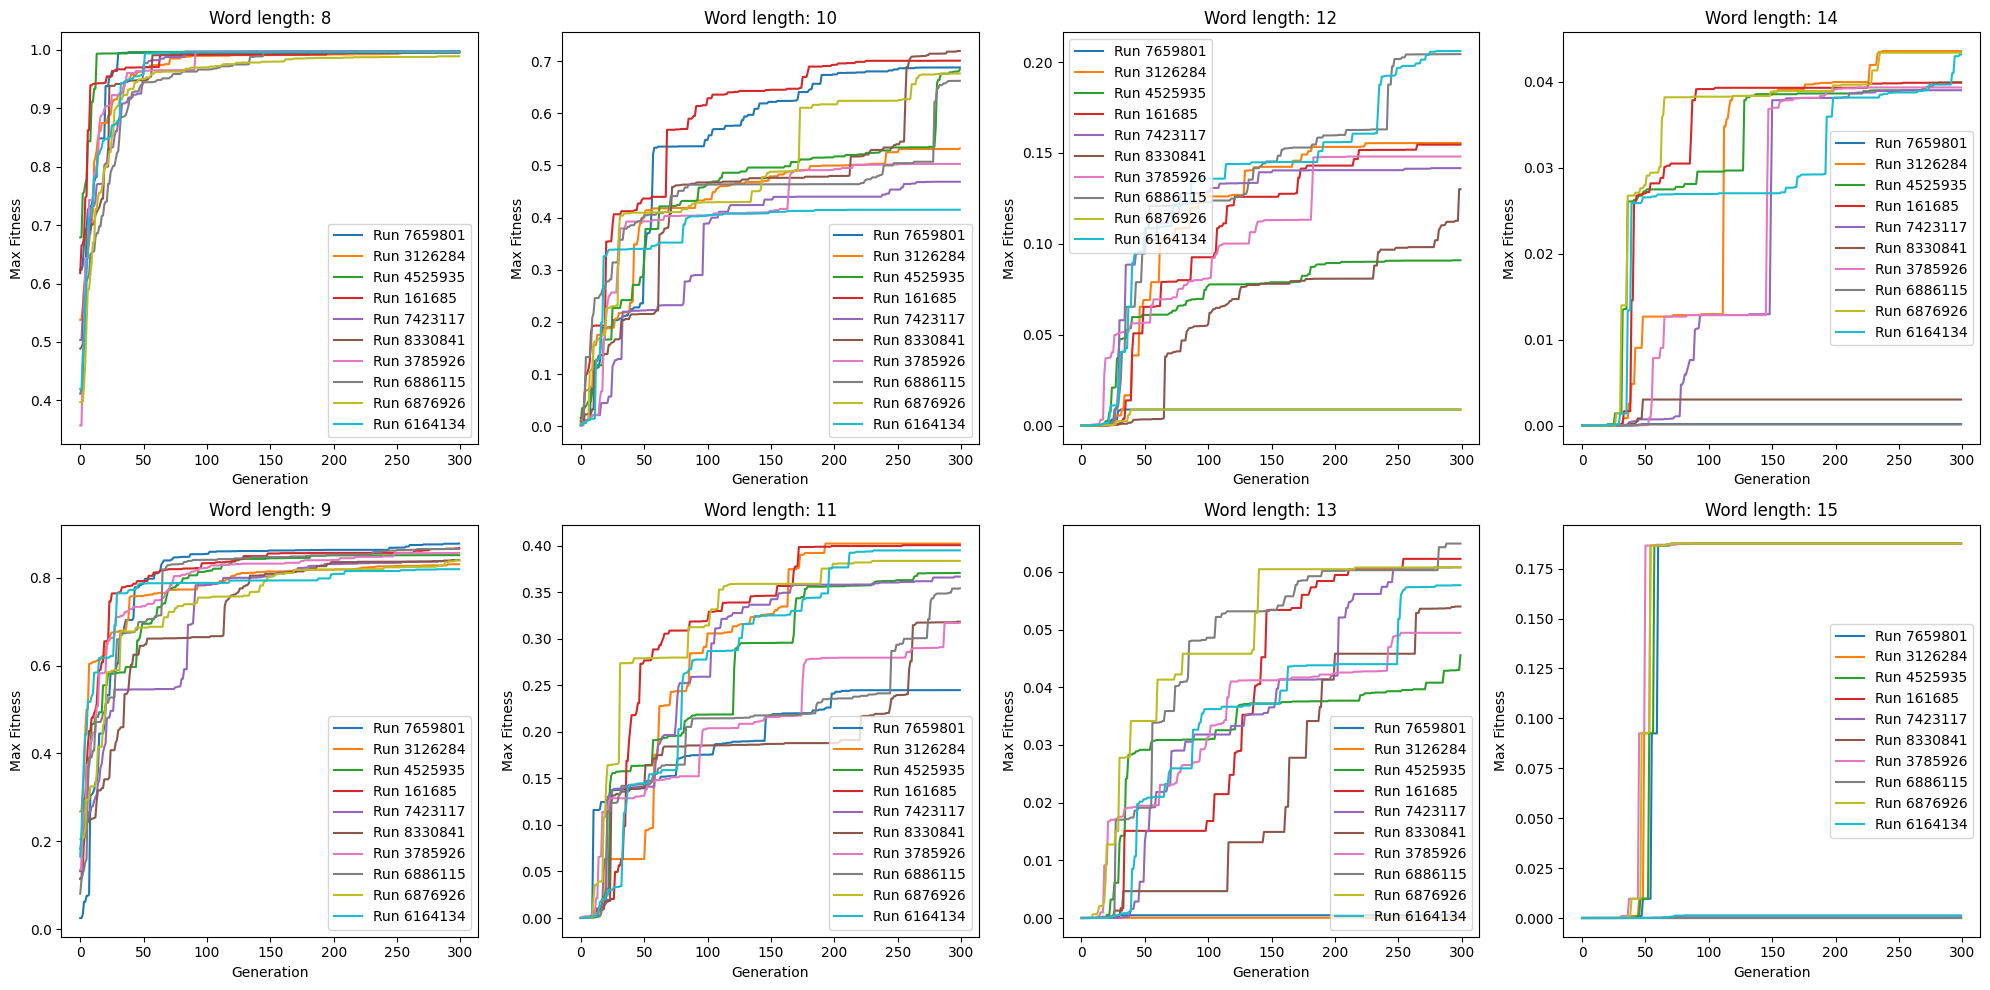
\includegraphics[width=\textwidth]{sampleteaser}
%   \caption{Seattle Mariners at Spring Training, 2010.}
%   \Description{Enjoying the baseball game from the third-base
%   seats. Ichiro Suzuki preparing to bat.}
%   \label{fig:teaser}
% \end{teaserfigure}

% \received{\today}
% \received[revised]{12 March 2009}
% \received[accepted]{5 June 2009}

%%
%% This command processes the author and affiliation and title
%% information and builds the first part of the formatted document.
\maketitle

\section{Introduction}
During Information Security Red Team operations, it is common to encounter password hashes when performing offensive tasks.
For example, during post-exploitation activities in an Active Directory environment, it is possible to extract NTLM hashes from the domain controller.
In order to recover the original password from these hashes, it is necessary to use password cracking tools.
One of the most popular tools for this task is Hashcat \cite{hashcat},
that supports a wide range of hash types and attack modes and make efficient use of the graphics card (GPU) to improve the speed of the attacks.

Hashcat works by receiving a list of target hashes and a list of candidate passwords.
For each candidate password, Hashcat applies a hash function to it and compares the result with the target hashes.
If the result matches any of the target hashes, the password is considered cracked.
Otherwise, the process continues with the next candidate password.
The different attack modes in Hashcat differ in the way the candidate passwords are generated, and can be summarized as follows:

\begin{itemize}
  \item \textbf{Dictionary attack}: Hashcat uses a wordlist of candidate passwords, called a dictionary, to try to recover the passwords.
These attacks can be further extended by using rules to modify the candidate passwords.

  \item \textbf{Mask attack}: Hashcat generates candidate passwords based on a mask or list of masks.
These masks define the structure of the candidate passwords, with each character in the mask representing a character in the candidate password.

  \item \textbf{Hybrid attack}: Hashcat combines the dictionary and mask attacks, generating candidate passwords by applying masks either before or after the words in the dictionary.
\end{itemize}

The most difficult part of the password cracking process is generating effective candidate passwords.
On one hand, it is desired to generate as many candidate passwords as possible, since that increases the chances one of them will match the target hash.
On the other, hand generating too many candidate passwords and calculating their respective hashes can be computationally expensive, slowing down the cracking process.
For this reason, the main goal of password cracking is to generate the most effective candidate passwords, that is, the ones that are more likely to match the target hashes.

When working with the dictionary attack mode, it is common to use wordlists available on the internet.
These wordlists are usually created from real passwords leaked in data breaches, and therefore should contain good candidate passwords.
Alternatively, it is possible to create custom wordlists by combining existing wordlists or using tools like CUPP \cite{cupp} to generate them.
Lastly, it is possible to use rules to modify the candidate passwords, for example by adding numbers or special characters to them.

However, finding effective masks can be a more challenging process.
There are two large commonly available masks on the internet: the Corporate Masks \cite{corporate_masks} and the Extreme Breach Masks \cite{extreme_breach_masks}.
These masks are based on patterns observed in real-world passwords, but they might not be well optimized for recovering the most passwords in the shortest time.
This paper proposes evaluating these using genetic algorithms to optimize Hashcat masks, improving the efficiency of password cracking.
The GitHub repository for this project can be found at \url{https://github.com/RafaelDiasCampos/Genetic-Algorithm}.

\section{Hashcat Masks}
\label{sec:hashcat_masks}

Hashcat masks are strings that define the structure of the candidate passwords.
Each character in the mask represents a character in the candidate password, and can either represent a fixed character or a character set.
By default, Hashcat supports the following character sets:

\begin{itemize}
  \item \textbf{?d}: Digits from 0 to 9.
  \item \textbf{?l}: Lowercase letters from a to z.
  \item \textbf{?u}: Uppercase letters from A to Z.
  \item \textbf{?s}: Special characters.
  \item \textbf{?a}: All printable ASCII characters.
  \item \textbf{?b}: All ASCII characters.
\end{itemize}

For example, the mask \textbf{?l?l?l?l?l?l} represents a candidate password with 6 lowercase letters.
The mask \textbf{?d?d?d?d?d?d} represents a candidate password with 6 digits.
The mask \textbf{?l?d?l?d?l?d} represents a candidate password with 3 pairs of lowercase letters and digits.

For this paper, we consider masks that contain only the character sets \textbf{?d}, \textbf{?l}, \textbf{?u}, \textbf{?s}, and \textbf{?a}.
We also separate the masks based on their number of characters.
This way, each list of masks can be used to recover passwords of a specific length.

In this paper, we only consider masks that generate candidate passwords with a length between 8 and 15 characters.
These lengths were chosen because passwords shorter than 8 characters can often be cracked by doing an exhaustive search of every password candidate.
On the other hand, passwords longer than 15 characters are less common and take longer to crack, so they are not likely to be recovered in a reasonable time.

\section{Measuring Effectiveness of Masks}

Initially, it is necessary to decide how to evaluate the effectiveness of a list of masks.
The most obvious metric for measuring a mask effectiveness is the number of candidate passwords generated by the mask that match the target hashes.
However, this metric alone is not enough, since the goal is to generate the most candidate passwords in the shortest time possible.
Therefore, it is necessary to consider the time taken to generate the candidate passwords, which is proportional to the number of candidate passwords generated by that mask.

Additionally, it is important to consider that, in most real world scenarios, there is a limited for performing the brute force attacks.
However, at the same time, it is not an issue if a mask takes longer to execute than the available time, since it can be executed only partially.
At the same time, there should be a penalty for masks that exceed the maximum cost, to prioritize masks that fit the desired cost.
With that in mind, we decided to evaluate the masks based on the following metrics:

\begin{itemize}
  \item \textbf{Number of recovered password (matches)}: The number of candidate passwords generated by the mask that match the target hashes.
  \item \textbf{Cost}: The number of candidate passwords generated by the mask.
\end{itemize}

And on the following parameters:

\begin{itemize}
  \item \textbf{Maximum cost}: The maximum desired cost of the mask, that indicates the available time to run the attack.
  \item \textbf{Fitness penalty}: The percentage penalty applied to the fitness of the mask that exceeds the maximum cost.
\end{itemize}

Combining this, we arrived at the following fitness function for evaluating the masks:

\begin{equation}
\label{eq:fitness_function}
  \text{BaseFitness} = \text{Matches} / \text{Wordlist size}
\end{equation}
\begin{equation}
  \text{Fitness} = 
  \begin{cases}
    \text{BaseFitness}, & \text{if Cost} \leq \text{MaxCost} \\
    \text{BaseFitness} \times \frac{\text{MaxCost}}{\text{Cost}} \times ( 1 - \text{Penalty}), & \text{otherwise}
  \end{cases}
\end{equation}

\subsection{Calculating the number of matches}

One of the metrics used for calculating the fitness of a mask is the percentage of recovered passwords.
This step consists of using a wordlist to represent the passwords and measuring how many of them are generated by the mask.
In this paper, we used the Weakpass 4 wordlist \cite{weakpass4}, that can be freely obtained on the internet.
This list contains over 2 billion passwords obtained in data breaches, so it should be a good source of real passwords.

After obtaining the wordlist, we separated it into smaller wordlists, based on the password length.
With these smaller wordlists, it is now possible to load one of them into memory and iterate over the passwords and check if they are generated by the mask.
However, the large number of passwords in the wordlist makes this process computationally expensive.
Therefore, it is necessary to use a more efficient method to calculate the number of matches.

For this method, we first sorted each wordlist according to the following order:

\begin{itemize}
  \item \textbf{Lowercase letters}
  \item \textbf{Uppercase letters}
  \item \textbf{Digits}
  \item \textbf{Special characters}
\end{itemize}

With the sorted wordlists, it was possible to create a tree-like structure.
This was done by recursively performing a binary search on each wordlist, and storing the amount of passwords that match a certain mask.
The structure can be observed in figure AAA

The created structure allows for quickly calculating how many passwords a mask would crack, by traversing it and returning the value of the last node.
However, special care needs to be taken when dealing with a list of masks.
Multiple masks can generate the same password, so it is necessary to avoid counting them repeatedly.
To solve this issue, we used a set to store the last nodes reached by the masks, and later sum the values of these nodes to calculate the total number of matches.

With this method, it was possible to calculate the number of matches for a mask in a fraction of the time it would take to iterate over the wordlist.

\subsection{Calculating the cost}

The other metric used for calculating the fitness of a mask is the cost, that is, the number of candidate passwords generated by the mask.
Before calculating the cost of a mask, it is useful to calculate the cost of a character set, according to the number of characters in that set.
The table cost of each character set can be seen in table \ref{tab:cost}.

\begin{table}
  \caption{Cost of character sets}
  \label{tab:cost}
  \begin{tabular}{ccl}
    \toprule
    Character set & Cost & Comments\\
    \midrule
    \textbf{?d} & 10 & Digits from 0 to 9\\
    \textbf{?l} & 26 & Lowercase letters from a to z\\
    \textbf{?u} & 26 & Uppercase letters from A to Z\\
    \textbf{?s} & 33 & Special characters\\
    \textbf{?a} & 95 & All printable ASCII characters\\
    \bottomrule
  \end{tabular}
\end{table}

Since the masks generate a candidate password by combining the character sets, it is possible to calculate their cost by multiplying the cost of the character sets that compose it.

\subsection{Deciding the parameters}
\label{sec:deciding_parameters}

After designing a method for evaluating the fitness of a list of masks, it is necessary to decide the parameters used in the fitness function.
For this paper, we decided to use the following parameters:

\begin{itemize}
  \item \textbf{Maximum cost}: $5 \times 10^{15}$
  \item \textbf{Fitness penalty}: $0.05$
\end{itemize}

The maximum cost was chosen based on the runtime of about 10 hours in a computer with an Nvidia RTX 3070 Ti, measured at $76146.5$ MH/s with NTLM hashes.
The fitness penalty was chosen to only slightly penalize masks that exceed the maximum cost, since it is not a significant issue if a mask takes longer to execute than the available time.

\section{Calculating the fitness of the current methods}
\label{sec:calculating_baseline_fitness}

After designing a method for evaluating the fitness of a list of masks, it is necessary to calculate the fitness of the current used methods.
For this paper, we used the Corporate Masks \cite{corporate_masks} and the Extreme Breach Masks \cite{extreme_breach_masks}, as they are popular and freely available on the internet.
Both of these lists contains masks for passwords of different lengths, and we calculated the fitness of each mask in each list.

The Extreme Breach Masks contains different lists of masks, depending on their total runtime.
We used the largest one that is not compressed (14 1-year) because it includes all the masks in the previous lists.
Furthermore, we considered that the masks were sorted by their other of priority, since hashcat runs them in order.

For each password length decided in section \ref{sec:hashcat_masks}, we started calculating the fitness of the first mask in the list, using the parameters defined in section \ref{sec:deciding_parameters}.
We then added the second mask, and calculated the fitness of the combined list.
This process was repeated until the fitness dropped from one iteration to the next, indicating that the cost of the masks was larger than the desired maximum cost.
At this time, we returned the maximum fitness obtained, the masks that generated it, and their cost.

The results of calculations for the Corporate Masks can be seen in table \ref{tab:fitness_corporate}.
One additional observation is that there are not masks with 15 characters in the Corporate Masks, so we did not calculate the fitness for this length.
The results of calculations for the Extreme Breach Masks can be seen in table \ref{tab:fitness_extreme}.

\begin{table}
  \caption{Fitness of the Corporate Masks}
  \label{tab:fitness_corporate}
  \begin{tabular}{ccl}
    \toprule
    Length & Fitness & Cost \\
    \midrule
    8 & 0.972079 & 1605171098613760	 \\
    9 & 0.562294 & 4999603084300800 \\
    10 & 0.386915	 & 4998028389760000 \\
    11 & 0.208118	 & 4989306592000000 \\
    12 & 0.085927 & 4986552000000000	 \\
    13 & 0.032640	 & 4863360000000000 \\
    14 & 0.030719 & 4940000000000000 \\
    \bottomrule
  \end{tabular}
\end{table}

\begin{table}
  \caption{Fitness of the Extreme Breach Masks}
  \label{tab:fitness_extreme}
  \begin{tabular}{ccl}
    \toprule
    Length & Fitness & Cost \\
    \midrule
    8 & 0.999705 & 4999855044508416	 \\
    9 & 0.955987 & 4997928685184000 \\
    10 & 0.846787 & 4988401456221184 \\
    11 & 0.444393	 & 2834403868825600 \\
    12 & 0.175589 & 4411987691520000	 \\
    13 & 0.065720	 & 4394348800000000 \\
    14 & 0.034780	 & 1857600000000000 \\
    15 & 0.187582 & 3600000000000000 \\
    \bottomrule
  \end{tabular}
\end{table}

Analyzing these results, it is interesting to note that the Extreme Breach Masks have a much higher fitness for passwords of 9, 10, 11, 12 and 13 characters.
This indicates that the Extreme Breach Masks are more effective than the Corporate Masks for these lengths.
For passwords of lengths 8 and 14, both masks have similar fitness, indicating that they are both recover similar amounts of passwords.
However, for length 8, the Corporate Masks have a much lower cost, while for length 14, the Extreme Breach Masks have a lower cost.

\section{Genetic Algorithm}

After calculating the fitness of the current methods, it is necessary to design a method for optimizing the masks.
For this paper, we decided to use a genetic algorithm, since it is a popular method for optimizing problems with a large search space.
The genetic algorithm works by creating a population of candidate solutions, and then evolving them over multiple generations.
A simple general-purpose genetic algorithm was implemented using Python, that receives the following parameters:

\begin{itemize}
  \item \textbf{Population size}: The number of candidate solutions in each generation.
  \item \textbf{Generations}: The number of generations to evolve the candidates.
  \item \textbf{Crossover rate}: The probability of a candidate solution being crossed over.
  \item \textbf{Mutation rate}: The probability of a candidate solution being mutated.
  \item \textbf{Elitism}: The number of candidate solutions that are kept from one generation to the next.
  \item \textbf{Tournament size}: The number of candidate solutions that are selected to be part of the tournament selection step.
  \item \textbf{Initial population}: The initial candidate solutions.
  \item \textbf{Fitness function}: The function used to evaluate the fitness of a candidate solution.
  \item \textbf{Crossover function}: The function used to cross over two candidate solutions.
  \item \textbf{Mutation function}: The function used to mutate a candidate solution.
\end{itemize}

In order to use this algorithm, it is necessary to determine how an individual will be represented, implement the crossover and mutation genetic operators and the fitness function.
Lastly, it is necessary to define the parameters of the genetic algorithm, such as the population size, the number of generations, the crossover rate, the mutation rate, the elitism, and the tournament size.

The following sections will detail how these steps were performed.

\subsection{Representing the Individual}

An individual can be represented as the list of masks it contains.
For this we first created a MaskCharset enum that contains the character sets used in the masks.
Each charset contains their representation by hashcat, and their cost, as defined in table \ref{tab:cost}.

Following this, we created a Mask class that contains a list of MaskCharset, representing the mask.
This class contains a cost attribute, calculated by multiplying the cost of each MaskCharset in the list, and a method to generate the mask string, that is used by hashcat.

Finally, we created a MaskIndividual class that contains a list of Mask, representing the individual, and a parameter that defines the maximum number of masks that can be contained in the individual.
This class also contains a cost attribute, calculated by summing the cost of each Mask in the list.

\subsection{Genetic Operators}

The genetic operators used in the genetic algorithm are the crossover and mutation operators.
The crossover operator works by selecting two individuals from the population, and combining them to create a new individual.
The mutation operator works by selecting an individual from the population, and modifying it to create a new individual.

For the crossover operator, we generate the offspring by combining some masks from each parent.
We first decide on the amount of masks each children will have, by generating a random number between 1 and the maximum number of masks.
This number is generated following a normal distribution centered around the average number of masks in each parent.
We then select the masks from each parent, and combine them to create the children.

For the mutation operator, there are three possible mutations, that are randomly selected:

\begin{itemize}
  \item \textbf{Add mask}: Adds a random mask to the individual.
  \item \textbf{Remove mask}: Removes a random mask from the individual.
  \item \textbf{Mutate mask}: Mutates a random mask in the individual by changing one of its character sets.
\end{itemize}

\subsection{Fitness Function}

The fitness function used in the genetic algorithm is the same as the one used to calculate the fitness of the current methods.
This function receives an individual and calculates its fitness based on the number of matches and the cost of the individual, according to equation \ref{eq:fitness_function}.
The function also receives the maximum cost and the fitness penalty as parameters, with the values defined in section \ref{sec:deciding_parameters}.

\subsection{Deciding the Parameters}

After designing the genetic algorithm, it is necessary to decide the parameters used in the algorithm.
For this paper, we used the Python library Optuna \cite{optuna} to perform hyperparameter optimization.
This library works by performing multiple trials, each with a different set of parameters, and selecting the one that maximizes the fitness of the individuals.
We first chose the search space for each parameter when considering masks of length 10, and then ran the optimization process for 500 trials.
The search space for each parameter can be seen in table \ref{tab:search_space}.
The values chosen based on the optimization process can be seen in table \ref{tab:parameters}.

\begin{table}
  \caption{Search space for the parameters}
  \label{tab:search_space}
  \begin{tabular}{ccl}
    \toprule
    Parameter & Search space \\
    \midrule
    Population size & 10 to 300 \\
    Generations & 10 to 300 \\
    Crossover rate & 0.5 to 1.0 \\
    Mutation rate & 0.01 to 0.5 \\
    Elitism & 1 to 5 \\
    Tournament size & 3 to 5 \\
    Maximum masks & 5 to 30 \\
    \bottomrule
  \end{tabular}
\end{table}

\begin{table}
  \caption{Optimized parameters}
  \label{tab:parameters}
  \begin{tabular}{ccl}
    \toprule
    Parameter & Value \\
    \midrule
    Population size & 265 \\
    Generations & 300 \\
    Crossover rate & 0.675 \\
    Mutation rate & 0.235 \\
    Elitism & 5 \\
    Tournament size & 5 \\
    Maximum masks & 30 \\
    \bottomrule
  \end{tabular}
\end{table}

\subsection{Executing the Genetic Algorithm}

After deciding the parameters of the genetic algorithm, the next step is to execute it.
For this paper, we used the optimized parameters defined in table \ref{tab:parameters}, and ran the genetic algorithm 10 times for each password length, using fixed seeds.
The results of the genetic algorithm can be seen in table \ref{tab:fitness_genetic}.

\begin{table}
  \caption{Fitness of the Genetic Algorithm}
  \label{tab:fitness_genetic}
  \begin{tabular}{ccl}
    \toprule
    Length & Fitness & Cost \\
    \midrule
    8 & 0.998075 & 4998945864072960	 \\
    9 & 0.877505 & 4743958039584768 \\
    10 & 0.719535 & 4732924205039616 \\
    11 & 0.402315	 & 4917264338585600 \\
    12 & 0.206068 & 4858597775360000	 \\
    13 & 0.064911	 & 4917369600000000 \\
    14 & 0.043578	 & 4991200000000000 \\
    15 & 0.187582 & 4600000000000000 \\
    \bottomrule
  \end{tabular}
\end{table}

The progression of the fitness of the genetic algorithm can be seen in figures \ref{fig:fitness_genetic_8}, \ref{fig:fitness_genetic_9}, \ref{fig:fitness_genetic_10}, \ref{fig:fitness_genetic_11}, \ref{fig:fitness_genetic_12}, \ref{fig:fitness_genetic_13}, \ref{fig:fitness_genetic_14}, and \ref{fig:fitness_genetic_15}.
These figures show the fitness of the best individual in each generation, in each of the 10 executions of the algorithm for that password length.

\begin{figure}
  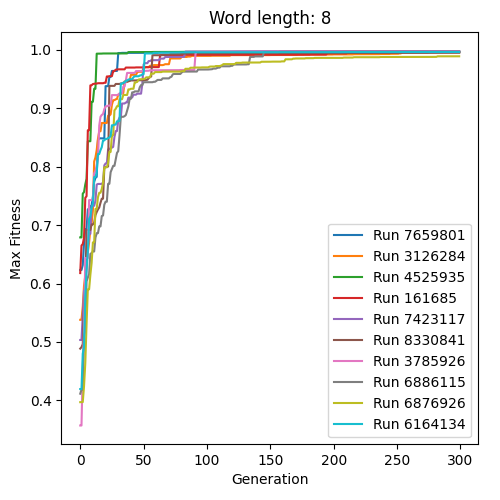
\includegraphics[width=\columnwidth]{genetic_results_8.png}
  \caption{Fitness of the Genetic Algorithm for passwords of length 8}
  \label{fig:fitness_genetic_8}
\end{figure}

\begin{figure}
  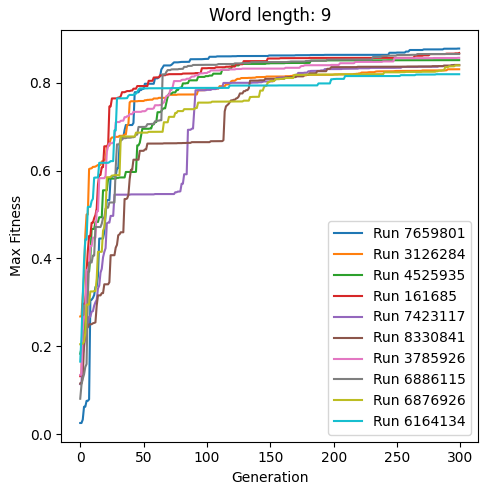
\includegraphics[width=\columnwidth]{genetic_results_9.png}
  \caption{Fitness of the Genetic Algorithm for passwords of length 9}
  \label{fig:fitness_genetic_9}
\end{figure}

\begin{figure}
  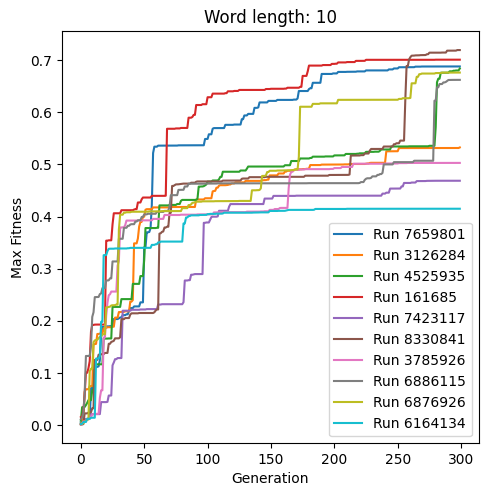
\includegraphics[width=\columnwidth]{genetic_results_10.png}
  \caption{Fitness of the Genetic Algorithm for passwords of length 10}
  \label{fig:fitness_genetic_10}
\end{figure}

\begin{figure}
  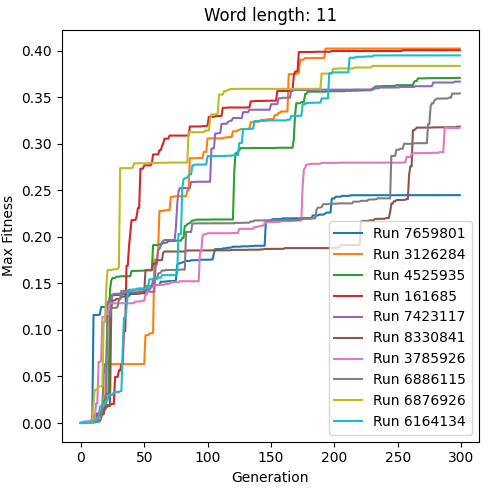
\includegraphics[width=\columnwidth]{genetic_results_11.png}
  \caption{Fitness of the Genetic Algorithm for passwords of length 11}
  \label{fig:fitness_genetic_11}
\end{figure}

\begin{figure}
  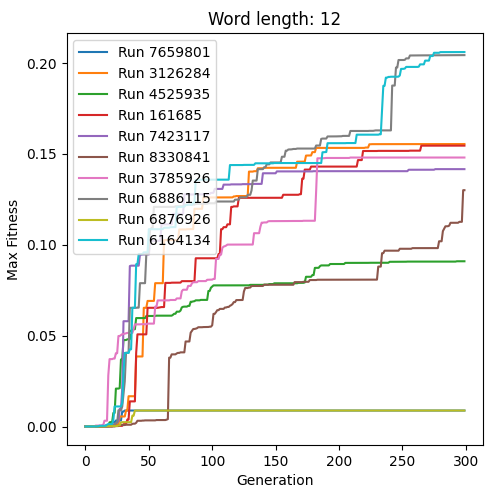
\includegraphics[width=\columnwidth]{genetic_results_12.png}
  \caption{Fitness of the Genetic Algorithm for passwords of length 12}
  \label{fig:fitness_genetic_12}
\end{figure}

\begin{figure}
  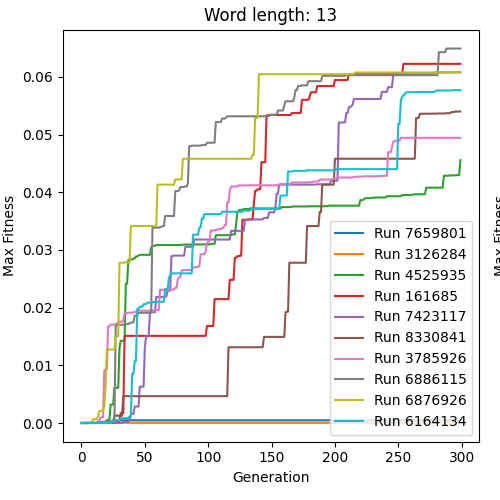
\includegraphics[width=\columnwidth]{genetic_results_13.png}
  \caption{Fitness of the Genetic Algorithm for passwords of length 13}
  \label{fig:fitness_genetic_13}
\end{figure}

\begin{figure}
  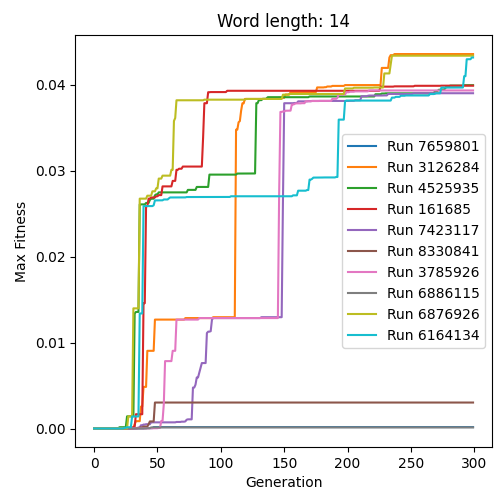
\includegraphics[width=\columnwidth]{genetic_results_14.png}
  \caption{Fitness of the Genetic Algorithm for passwords of length 14}
  \label{fig:fitness_genetic_14}
\end{figure}

\begin{figure}
  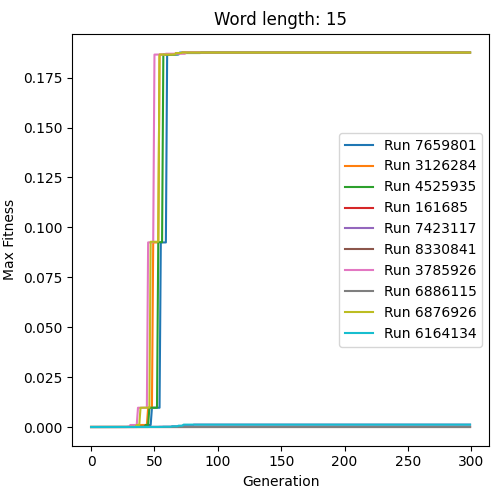
\includegraphics[width=\columnwidth]{genetic_results_15.png}
  \caption{Fitness of the Genetic Algorithm for passwords of length 15}
  \label{fig:fitness_genetic_15}
\end{figure}

It is possible to observe that the maximum fitness for word lengths 8 and 9 appear to have stabilized before the end of the execution.
On the other hand, the maximum fitness for word lengths 10, 11, 12, 13 and 14 were still unstable and could possibly get improved by running the algorithm for more generations.
Lastly, the maximum fitness for word length 15 appears to indicate that multiple executions arrived at the same result, possibly because there are not many passwords with that length.

Comparing the results obtained by the genetic algorithm with the results obtained by the current methods, it is possible to observe that the genetic algorithm was able to achieve a fitness greater than the Corporate Masks for all lengths.
The algorithm obtained a fitness similar to the Extreme Breach Masks for lengths 8, 13, and 15, and a fitness greater than the Extreme Breach Masks for lengths 12 and 14.
However, the algorithm obtained a fitness lower than the Extreme Breach Masks for lengths 9, 10 and 11.
A comparison of the final results can be seen in table \ref{tab:fitness_comparison}.
The masks generated by the genetic algorithm can be seen in the appendix.

\begin{table}
  \caption{Comparison of the fitness of the Genetic Algorithm with the current methods}
  \label{tab:fitness_comparison}
  \begin{tabular}{cccl}
    \toprule
    Length & Genetic Algorithm & Corporate & Extreme Breach \\
    \midrule
    8 & 0.998075 & 0.972079 & 0.999705 \\
    9 & 0.877505 & 0.562294 & 0.955987 \\
    10 & 0.719535 & 0.386915 & 0.846787 \\
    11 & 0.402315	 & 0.208118 & 0.444393 \\
    12 & 0.206068 & 0.085927 & 0.175589 \\
    13 & 0.064911	 & 0.032640 & 0.065720 \\
    14 & 0.043578	 & 0.030719 & 0.034780 \\
    15 & 0.187582 & - & 0.187582 \\
    \bottomrule
  \end{tabular}
\end{table}

\section{Conclusion}

This paper proposed evaluating the Corporate Masks and the Extreme Breach Masks using genetic algorithms to optimize Hashcat masks.
Initially, it is interesting to observe that the Corporate Masks obtained a significantly worse fitness than the Extreme Breach Masks for most password lengths, indicating that it is not very efficient for recovering passwords.
With the genetic algorithm, it was possible to generate masks that were later compared with the results obtained by the current methods.
After this step, it was observed that the genetic algorithm was able to achieve a fitness greater than the Corporate Masks for all lengths.
Furthermore, the algorithm obtained a fitness similar to the Extreme Breach Masks for lengths 8, 13, and 15, and a fitness greater than the Extreme Breach Masks for lengths 12 and 14.
However, it obtained a fitness lower than the Extreme Breach Masks for lengths 9, 10 and 11.

We can conclude that the results obtained by the genetic algorithm can be used to improve the efficiency of password cracking, by generating more effective masks for some specific lengths.
However, for some lengths, the Extreme Breach Masks are still more effective and should be used instead.
It is possible that the genetic algorithm could achieve better results by running for more generations, or by using a different choice of parameters or genetic operators.
Lastly, different methods could be used to search for the optimal masks, such as simulated annealing or particle swarm optimization.


%%
%% The next two lines define the bibliography style to be used, and
%% the bibliography file.
\bibliographystyle{ACM-Reference-Format}
\bibliography{bibliography}

%%
%% If your work has an appendix, this is the place to put it.
\appendix

\section{Masks generated by the Genetic Algorithm}

The masks generated by the genetic algorithm are included in the following subsections.

\subsection{Masks for passwords of length 8}
\lstinputlisting{../results/masks/masks_8.txt}

\subsection{Masks for passwords of length 9}
\lstinputlisting{../results/masks/masks_9.txt}

\subsection{Masks for passwords of length 10}
\lstinputlisting{../results/masks/masks_10.txt}

\subsection{Masks for passwords of length 11}
\lstinputlisting{../results/masks/masks_11.txt}

\subsection{Masks for passwords of length 12}
\lstinputlisting{../results/masks/masks_12.txt}

\subsection{Masks for passwords of length 13}
\lstinputlisting{../results/masks/masks_13.txt}

\subsection{Masks for passwords of length 14}
\lstinputlisting{../results/masks/masks_14.txt}

\subsection{Masks for passwords of length 15}
\lstinputlisting{../results/masks/masks_15.txt}

\end{document}
\endinput